\documentclass[12pt]{standalone}
\usepackage{tikz}
\usetikzlibrary{patterns} % calc, arrows.meta, decorations.pathreplacing}
\begin{document}
%lwarp%\begin{lateximage}[an oval X broken into two pieces U and V separated by a dashed gap with g=0 on U and g=1 on V][][width: 65\%;]
		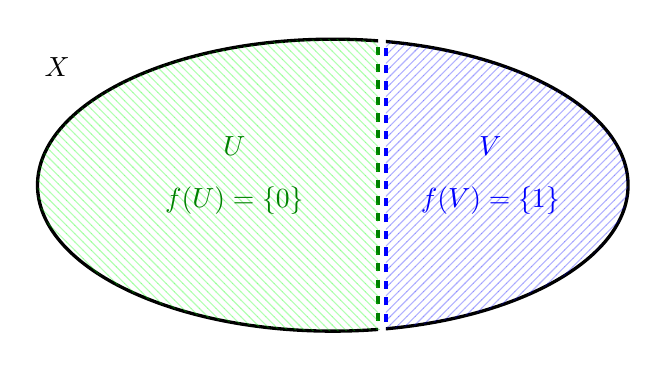
\begin{tikzpicture}[xscale=1.25]
			\path[save path=\leftrect] (-3.1,-1.95) rectangle (0.46,2);
			\path[save path=\rightrect] (0.54,-1.95) rectangle (3.1,2);
			\path[save path=\bigellipse] (0,0) circle[x radius=3, y radius=1.854];
			\begin{scope}
				\clip[use path=\leftrect];
				\draw[very thick, black, use path=\bigellipse];
			\end{scope}
			\begin{scope}
				\clip[use path=\rightrect];
				\draw[very thick, black, use path=\bigellipse];
			\end{scope}
			\begin{scope}
				\clip[use path=\bigellipse];
				\draw[very thick, green!50!black, dashed, use path=\leftrect];
				\draw[very thick, blue, dashed, use path=\rightrect];
				\fill[pattern color=green, pattern=north west lines, opacity=0.3, use path=\leftrect];
				\fill[pattern color=blue, pattern=north east lines, opacity=0.3, use path=\rightrect];
				\node[green!50!black] at (-1,0.5) {$U$};
				\node[green!50!black] at (-1,-0.2) {$f(U)=\{0\}$};
				\node[blue] at (1.6,0.5) {$V$};
				\node[blue] at (1.6,-0.2) {$f(V)=\{1\}$};
			\end{scope}
			\node[black] at (-2.8,1.5) {$X$};
		\end{tikzpicture}
\end{document}
